\documentclass[11pt,a4paper]{article}
\usepackage[margin=24mm]{geometry}
\usepackage[T1]{fontenc}
\usepackage{lmodern,microtype}
\usepackage{amsmath,amssymb,amsthm,mathtools,mathrsfs}
\usepackage{booktabs,array}
\usepackage{xcolor,tikz}
\usetikzlibrary{arrows.meta,positioning,calc,shapes.geometric}
\usepackage{placeins,float,needspace}
\usepackage[hidelinks]{hyperref}
\usepackage[nameinlink,noabbrev]{cleveref}

\definecolor{accent}{HTML}{284F68}
\definecolor{wash}{HTML}{EFF5F8}
\definecolor{green}{HTML}{3F7058}
\definecolor{greenwash}{HTML}{ECF4EE}
\definecolor{ochre}{HTML}{916A39}
\definecolor{ochrewash}{HTML}{F8F1E6}
\tikzset{
 flow/.style={-{Latex[length=2mm]},draw=accent,thick},
 card/.style={draw=accent,fill=wash,rounded corners=2pt,
     align=center,inner sep=6pt,font=\small},
 good/.style={card,draw=green,fill=greenwash},
 prior/.style={card,draw=ochre,fill=ochrewash},
 decision/.style={diamond,aspect=2.5,draw=accent,fill=wash,
     align=center,inner sep=3pt,font=\small}
}
\newtheorem{theorem}{Theorem}[section]
\newtheorem{proposition}[theorem]{Proposition}
\newtheorem{lemma}[theorem]{Lemma}
\newtheorem{corollary}[theorem]{Corollary}
\theoremstyle{definition}
\newtheorem{definition}[theorem]{Definition}
\newtheorem{construction}[theorem]{Construction}
\theoremstyle{remark}
\newtheorem{remark}[theorem]{Remark}
\crefname{construction}{construction}{constructions}
\Crefname{construction}{Construction}{Constructions}
\newcommand{\F}{\mathbb F_2}
\newcommand{\wt}{\operatorname{wt}}
\newcommand{\css}{\operatorname{wt}_{\mathrm{CSS}}}
\newcommand{\Q}{\mathcal Q}
\newcommand{\St}{\mathcal S}
\newcommand{\Norm}{\mathcal N(\mathcal S)}
\newcommand{\Hist}{\mathcal H}
\newcommand{\Safe}{\mathcal C_{\mathrm{safe}}}
\newcommand{\DPrep}{\mathsf{DPrep}}
\newcommand{\SE}{\mathsf{SE}}
\newcommand{\ket}[1]{\lvert #1\rangle}
\setlength{\parskip}{4pt}
\setlength{\emergencystretch}{2em}
\allowdisplaybreaks
\hypersetup{
 pdftitle={Adaptive Steane error correction without postselection},
 pdfsubject={Deterministic state preparation and minimal adaptive actions}
}
\title{Adaptive Steane error correction without postselection\\
\large From the measurement record to the next minimal action}
\author{Working mathematical proposal}
\date{17 October 2026}

\begin{document}
\maketitle
\begin{abstract}
An adaptive Steane cycle should use every prepared ancilla, including
flagged ones, and finish with a correction satisfying the two EC
conditions. We develop the protocol as a sequence of questions: what
errors can each extraction introduce, what does its record establish, when
is a common correction available, and which extraction should be run next?
Compatible fault histories give an exact stopping rule and a finite
optimization of the remaining work. Deterministic fault-tolerant state
preparation provides a direct two-extraction construction. For a family of
deterministic preparations with protection through $b$ faults at label
$2b+1$, a certified lower bound $L$ on spent faults permits the second
label $d-2L$. The same history-based stopping rule also applies to the
earlier nondeterministic preparation circuits when all their outputs are
retained. A fault-charging condition bounds the number of rounds, and
acceptance probabilities give recursions for the expected gadget count.
\end{abstract}

\section{The correction problem}
\label{sec:model}

\begin{definition}[Code, errors, and fault count]
Let $\Q$ be an $[[n,k,d]]$ CSS code with $d=2t+1$ and stabilizer group
$\St$. The data start in an arbitrary encoded state $\ket\psi$, possibly
entangled with a reference, followed by
\[
 E_{\mathrm{in}}=X(u)Z(v),\qquad u,v\in\F^n.
\]
We use
\begin{equation}
 \css(X(x)Z(z))=\max\{\wt(x),\wt(z)\},\qquad
 r=\css(E_{\mathrm{in}}).
 \label{eq:metric}
\end{equation}
Vectors add modulo two and Pauli phases are suppressed. An internal fault
is a Pauli fault at an elementary circuit location. The number $s$ of
internal faults is summed over the entire executed cycle.
\end{definition}

\begin{remark}[Fault model and corrections]
The propagation model first places faults in ancilla preparations and takes
the couplings and readout to be ideal. The compatible-history construction
also allows faults in gates, measurements, resets, and data idles.
\Cref{sec:fullnoise} gives the corresponding extension of the
two-extraction construction. Corrections are Pauli-frame updates.
Each faulty location contributes one to $s$, including a location carrying
a $Y$ fault.
\end{remark}

\begin{lemma}[CSS correction radius]
The code corrects every error of CSS weight at most $t$.
\end{lemma}
\begin{proof}
Decode the components separately. The product of two errors of CSS weight
at most $t$ has each component of weight at most $2t<d$. If that product
is in the normalizer, each component is a stabilizer. Thus two errors with
the same syndrome have the same logical effect.
\end{proof}

\begin{definition}[A cycle without postselection]
A cycle begins with Z-SE and retains every preparation flag and syndrome
outcome. It may perform further extractions in either basis. Every branch
ends with a Pauli correction and an output data block. Every prepared
ancilla is used, with any assigned preparation correction tracked in the
Pauli frame.
\end{definition}

\begin{definition}[The two EC conditions]
Let $\Pi_j^{\mathrm{CSS}}$ project onto the span of $E\ket\psi$ with
$\ket\psi\in\Q$ and $\css(E)\leq j$, and let $\mathcal D$ be a fixed
ideal decoder for this CSS error set through radius $t$. We require the
CSS form of Gottesman's EC conditions
\cite[Definition~5]{gottesman}:
\begin{description}
 \item[EC A:] For every input and every $s\leq t$ internal faults, the
 output is supported in $\operatorname{im}\Pi_s^{\mathrm{CSS}}$.
 \item[EC B:] Whenever $r+s\leq t$, ideal decoding after the cycle
 gives the same logical state as ideal decoding before it.
\end{description}
\label[definition]{def:EC}
\end{definition}

\begin{remark}[Two roles for the input]
EC A asks that the output be close to some codeword, for every input
syndrome sector. EC B additionally asks for the correct logical codeword
when the incoming error and internal faults satisfy $r+s\leq t$.
The CSS filter in \cref{def:EC} makes the componentwise metric explicit.
The same two roles appear in the flag-EC formulation of
\cite[Definition~1]{chao}.
\end{remark}

\begin{definition}[Residual-error distances]
For a data Pauli $P$, define
\begin{align}
 \mu(P)&=\min_{N\in\Norm}\css(PN),\label{eq:mu}\\
 \nu(P)&=\min_{S\in\St}\css(PS).\label{eq:nu}
\end{align}
Thus $\mu$ measures the distance to some codeword sector, while $\nu$
retains the logical action relative to the original encoded state.
\end{definition}

\begin{proposition}[Pauli form of the EC conditions]
\label[proposition]{prop:paulitests}
Suppose a history with incoming weight $r$ and $q\leq t$ internal faults
leaves the data in $P\ket\psi$. A correction $C$ satisfies the required
conditions for that history precisely when
\begin{align}
 \mu(CP)&\leq q &&\text{for EC A},\tag{A}\label{eq:testA}\\
 \nu(CP)&\leq q &&\text{if }r+q\leq t.\tag{B}\label{eq:testB}
\end{align}
Here (B), together with (A), is the EC B requirement.
\end{proposition}
\begin{proof}
Condition (A) says that $CP=RN$ for some $\css(R)\leq q$ and
$N\in\Norm$. Ideal decoding removes $R$ and retains the logical action of
$N$. In the regime $r+q\leq t$, preserving the original logical state for
every $\ket\psi$ is equivalent to $N\in\St$, which is (B).
\end{proof}

\begin{remark}[The fault count at an endpoint]
Each history carries its own value of $q$ in
\cref{prop:paulitests}. In particular, a zero-fault cycle returns a
codeword, and it returns the original codeword for every correctable
zero-fault input.
\end{remark}

\section{A Steane extraction as an error transition}
\label{sec:coupling}

We next describe exactly which data errors and observations pass from one
stage to the next.

\begin{definition}[The two extraction bases]
Let $H_Z,H_X$ contain the supports of the Z and X stabilizer generators.
Z-SE measures the X-error syndrome $H_Zx$; X-SE measures the Z-error
syndrome $H_Xz$. Write $\ket{\overline{+^k}}$ and
$\ket{\overline{0^k}}$ for the encoded all-plus and all-zero logical states
of one $n$-qubit ancilla block. The Steane couplings are
\begin{equation}
\begin{array}{ccl}
 \text{Z-SE:}&\operatorname{CNOT}_{D\to A},&
 A=\ket{\overline{+^k}},\quad \text{measure }A\text{ in Z},\\[2pt]
 \text{X-SE:}&\operatorname{CNOT}_{A\to D},&
 A=\ket{\overline{0^k}},\quad \text{measure }A\text{ in X}.
\end{array}
\label{eq:ancillas}
\end{equation}
\end{definition}

\begin{remark}[Logical-state convention]
These states make the logical coupling act trivially on the data: a
logical plus target is invariant under the data-controlled X, and a
logical zero control leaves the target unchanged. These are the ancilla
labels used in \cref{fig:two}, with the CNOT directions of
\texttt{adaptive-steane.tikz}; see also
\cite[Sec.~4.4]{gottesman}.
\end{remark}

\begin{figure}[H]
\centering
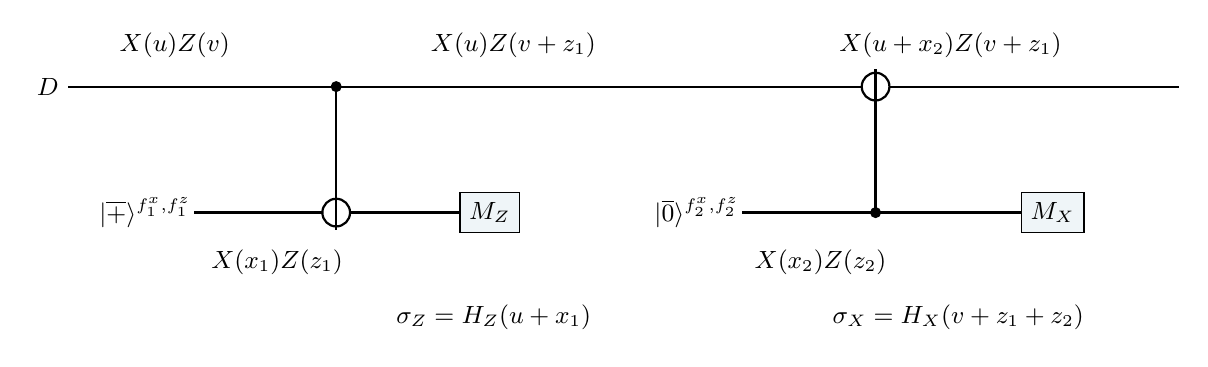
\begin{tikzpicture}[x=1cm,y=1cm,>=Latex,font=\small,
 labelbox/.style={fill=white,inner sep=2pt}]
 \draw[thick] (0,0)--(14.1,0);
 \node[anchor=east] at (0,0) {$D$};
 \node[labelbox] at (1.35,.52) {$X(u)Z(v)$};
 \node[labelbox] at (5.65,.52) {$X(u)Z(v+z_1)$};
 \node[labelbox] at (11.2,.52) {$X(u+x_2)Z(v+z_1)$};
 \draw[thick] (0.4,-1.6)--(5.25,-1.6);
 \node[anchor=west,fill=white,inner sep=1pt] at (.35,-1.6)
     {$\ket{\overline+}^{f_1^x,f_1^z}$};
 \fill (3.4,0) circle (2pt);
 \draw[thick] (3.4,0)--(3.4,-1.6);
 \draw[thick,fill=white] (3.4,-1.6) circle (5pt);
 \draw[thick] (3.4,-1.82)--(3.4,-1.38);
 \node[draw,fill=wash,minimum width=.65cm,minimum height=.5cm]
     at (5.35,-1.6) {$M_Z$};
 \node[anchor=north] at (2.65,-1.95) {$X(x_1)Z(z_1)$};
 \node[anchor=north,align=center] at (5.4,-2.65)
     {$\sigma_Z=H_Z(u+x_1)$};
 \draw[thick] (7.45,-1.6)--(12.4,-1.6);
 \node[anchor=west,fill=white,inner sep=1pt] at (7.4,-1.6)
     {$\ket{\overline0}^{f_2^x,f_2^z}$};
 \fill (10.25,-1.6) circle (2pt);
 \draw[thick] (10.25,-1.6)--(10.25,0);
 \draw[thick,fill=white] (10.25,0) circle (5pt);
 \draw[thick] (10.25,-.22)--(10.25,.22);
 \node[draw,fill=wash,minimum width=.65cm,minimum height=.5cm]
     at (12.5,-1.6) {$M_X$};
 \node[anchor=north] at (9.55,-1.95) {$X(x_2)Z(z_2)$};
 \node[anchor=north,align=center] at (11.3,-2.65)
     {$\sigma_X=H_X(v+z_1+z_2)$};
\end{tikzpicture}
\caption{The two Steane extractions before syndrome corrections. The
ancilla states use the conventional logical labels for the displayed CNOT
directions. Each superscript $f_i^x,f_i^z$ denotes recorded preparation
flags. All syndrome values and propagated errors are retained.}
\label{fig:two}
\end{figure}

\begin{lemma}[The first two extractions]
\label[lemma]{lem:two-transitions}
Suppose the first and second prepared ancillas have boundary errors
$X(x_1)Z(z_1)$ and $X(x_2)Z(z_2)$, respectively. Before syndrome
corrections, the recorded syndromes and data errors are
\begin{align}
 \sigma_Z&=H_Z(u+x_1),&
 E_D^{(1)}&=X(u)Z(v+z_1),\label{eq:first}\\
 \sigma_X&=H_X(v+z_1+z_2),&
 E_D^{(2)}&=X(u+x_2)Z(v+z_1).\label{eq:second}
\end{align}
\end{lemma}
\begin{proof}
In the first CNOT layer, an ancilla X error changes its Z readout and an
ancilla Z error propagates to the data. In the second layer, an ancilla Z
error changes its X readout and an ancilla X error propagates to the data.
Substituting the data error after the first layer gives the second line.
\end{proof}

\begin{remark}[What is observed]
The physical readout contains a random classical codeword plus the error
vector. Applying $H_Z$ or $H_X$ gives the syndrome in
\cref{lem:two-transitions}. Thus the observations are the flags and these
syndromes, together with any additional readout bits retained by the
decoder.
\end{remark}

\begin{lemma}[Recursive transition]
\label[lemma]{lem:transition}
If the current data error has supports $(x,z)$ and a fresh ancilla has
boundary supports $(\xi,\zeta)$, the next extraction has the response
\begin{equation}
\begin{array}{c|c|c}
 \text{action}&\text{recorded syndrome}&\text{new data supports}\\
 \hline
 Z\text{-SE}&H_Z(x+\xi)&(x,\ z+\zeta)\\
 X\text{-SE}&H_X(z+\zeta)&(x+\xi,\ z).
\end{array}
\label{eq:recurrence}
\end{equation}
Known frame corrections are incorporated in the supports and readout
processing.
\end{lemma}
\begin{proof}
Apply the same CNOT propagation used in \cref{lem:two-transitions} to
the current supports instead of the initial ones.
\end{proof}
\FloatBarrier

\section{What the measurement record establishes}
\label{sec:histories}

\begin{definition}[Actions and records]
An extraction action is $a=(B,\delta)$, where $B\in\{Z,X\}$ is the measured
stabilizer basis and $\delta$ identifies a preparation and its associated
coupling and readout. The code distance is always $d$.
The complete record $R$ contains the chosen actions, their flags and
retained readouts, and all known frame updates.
\end{definition}

\begin{definition}[Compatible histories]
Let
\begin{equation}
 \Hist(R)=\{h=(E_{\mathrm{in}},F,P_h,r_h,q_h):
          h\text{ produces }R,\ q_h\leq t\}.
 \label{eq:hist}
\end{equation}
Here $F$ specifies the internal fault locations and their Pauli effects,
$q_h=|F|$, $r_h=\css(E_{\mathrm{in}})$, and $P_h$ is the current data
Pauli relative to the original encoded state.
All incoming Pauli errors are included for EC A. The histories also
carrying a logical-preservation requirement at the current endpoint form
\begin{equation}
 \Hist_B(R)=\{h\in\Hist(R):r_h+q_h\leq t\}.
 \label{eq:HB}
\end{equation}
\end{definition}

\begin{construction}[Updating the compatible set]
For each candidate history, enumerate the new preparation responses
$(\ell,f,\xi,\zeta)$, where $\ell$ is its fault count. Use
\cref{lem:transition} to compute the next syndrome and data supports.
Keep responses matching the new observations with $q_h+\ell\leq t$,
and update $q_h$ to $q_h+\ell$. The initial data supports are $(u,v)$.
For a complete noisy extraction, the same construction propagates faults
through its full circuit.
\label[construction]{con:update}
\end{construction}

\begin{lemma}[The true history survives]
\label[lemma]{lem:true}
For every executed prefix with at most $t$ faults, its true input Pauli,
fault history, and current data Pauli belong to $\Hist(R)$.
\end{lemma}
\begin{proof}
The initial set contains the true input. At each update, the actual new
faults produce the observed flags and syndrome and satisfy the total
fault-count bound. Induction proves the claim.
\end{proof}

\begin{figure}[H]
\centering
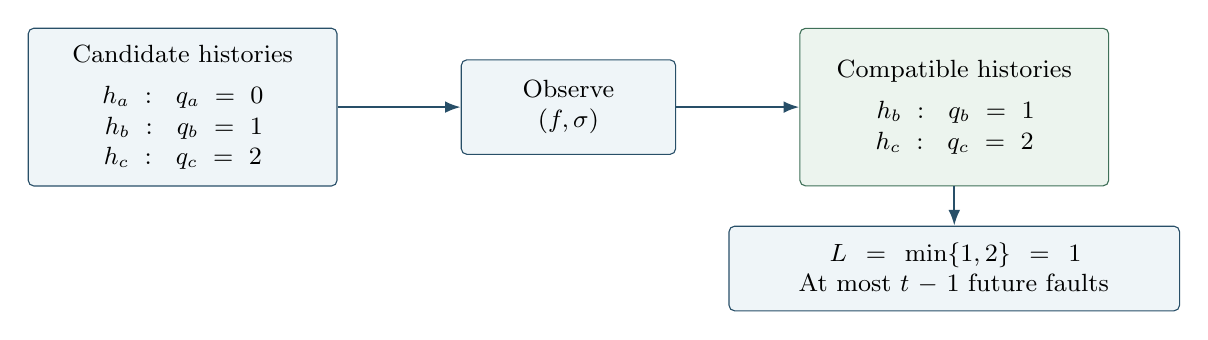
\begin{tikzpicture}[>=Latex,font=\small]
 \node[card,text width=3.5cm,minimum height=2.0cm] (before) at (0,0)
   {Candidate histories\\[4pt]
    $h_a:\ q_a=0$\\
    $h_b:\ q_b=1$\\
    $h_c:\ q_c=2$};
 \node[card,text width=2.3cm,minimum height=1.2cm] (record) at (4.9,0)
   {Observe\\$(f,\sigma)$};
 \node[good,text width=3.5cm,minimum height=2.0cm] (after) at (9.8,0)
   {Compatible histories\\[4pt]
    $h_b:\ q_b=1$\\
    $h_c:\ q_c=2$};
 \draw[flow] (before)--(record);
 \draw[flow] (record)--(after);
 \node[card,text width=5.3cm] (budget) at (9.8,-2.05)
   {$L=\min\{1,2\}=1$\\
    At most $t-1$ future faults};
 \draw[flow] (after.south)--(budget.north);
\end{tikzpicture}
\caption{A schematic record narrows the compatible histories. Several
fault counts may survive while giving the same useful lower bound on
spent faults.}
\label{fig:histories}
\end{figure}

\begin{definition}[Spent and remaining fault budgets]
For a nonempty compatible set, define
\begin{equation}
 L(R)=\min_{h\in\Hist(R)}q_h,\qquad b(R)=t-L(R).
 \label{eq:remaining}
\end{equation}
\end{definition}

\begin{lemma}[Budget update]
\label[lemma]{lem:budget}
Along a reachable branch, $L(R)$ is nondecreasing. At most $b(R)$ further
faults can occur in an execution with total count at most $t$.
History $h$ has the sharper future bound $t-q_h$ for EC A and, when
$r_h+q_h\leq t$, the bound $t-r_h-q_h$ for EC B.
\end{lemma}
\begin{proof}
An extended history restricts to a compatible prefix and adds a
nonnegative number of faults. Every prefix count is at least $L(R)$.
Subtracting each prefix count from the corresponding total bound gives
the stated future bounds.
\end{proof}

\begin{proposition}[A bound from preparation flags]
\label[proposition]{prop:flags}
For a preparation whose flags are independent of the data, set
\begin{equation}
 e_i(f_i)=\min\{|F_i|:F_i\text{ produces }f_i\}.
 \label{eq:localminimum}
\end{equation}
After disjoint preparations $1,\ldots,j$, the value
$\sum_{i=1}^j e_i(f_i)$ is a certified lower bound on spent faults.
A joint flag pattern can be replaced by any recorded subset to obtain
a valid, possibly smaller, lower bound.
\end{proposition}
\begin{proof}
Every compatible history uses at least $e_i(f_i)$ faults in preparation
$i$. Its total count is the sum over disjoint preparations.
\end{proof}

\begin{remark}[Typed flags]
If $e_i^x$ and $e_i^z$ are computed from two flag subsets in the same
preparation, their maximum is a valid combined bound. A joint minimization
as in \eqref{eq:localminimum} accounts for faults, such as a $Y$ fault,
that contribute to both subsets. Because preparation flags are independent
of the incoming data, these bounds apply throughout the EC A input domain.
\end{remark}
\FloatBarrier

\section{When the cycle can finish}
\label{sec:stop}

\begin{definition}[Common safe corrections]
For each history, let
\[
 \mathcal A_h=\{C:\mu(CP_h)\leq q_h\},\qquad
 \mathcal B_h=\{C:\nu(CP_h)\leq q_h\}.
\]
The corrections compatible with the complete record are
\begin{equation}
 \boxed{\displaystyle
 \Safe(R)=
 \bigcap_{h\in\Hist(R)}\mathcal A_h
 \ \cap\!
 \bigcap_{h\in\Hist_B(R)}\mathcal B_h.}
 \label{eq:safe}
\end{equation}
\end{definition}

\begin{proposition}[Exact stopping rule]
\label[proposition]{prop:stop}
For a nonempty compatible set, the cycle can finish now with a Pauli
correction satisfying both EC conditions for every compatible history if
and only if $\Safe(R)\ne\varnothing$.
\end{proposition}
\begin{proof}
A correction in the intersection obeys both history-dependent tests of
\cref{prop:paulitests}. Conversely, a correction obeying those tests for
every compatible history belongs to every set in the intersection.
\end{proof}

\begin{corollary}[Minimal terminal action]
Whenever $\Safe(R)\ne\varnothing$, a frame update by any
$C\in\Safe(R)$ completes the cycle. When $\Safe(R)=\varnothing$,
a protocol using terminal Pauli corrections requires another extraction.
\end{corollary}
\begin{proof}
This is \cref{prop:stop} applied to the two possible outcomes of the
intersection test.
\end{proof}

\begin{remark}[Choosing the next basis]
The next basis follows the unresolved error information. After Z-SE,
another Z-SE can refine the X-error syndrome $H_Z(u+x_1)$; an X-SE can
resolve the propagated Z component $v+z_1$. The complete record determines
whether either refinement is needed. The same stopping test handles
zero and nonzero flag outcomes.
\end{remark}

\begin{figure}[H]
\centering
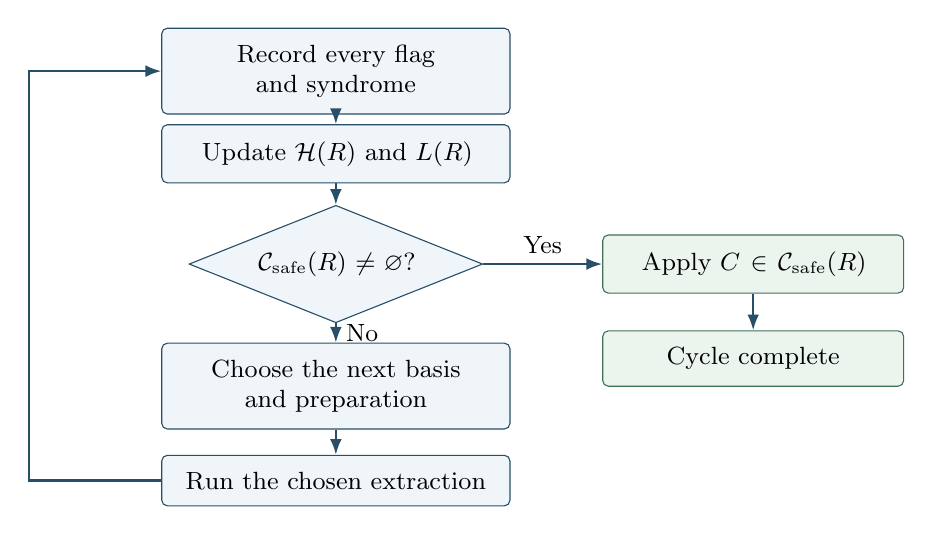
\begin{tikzpicture}[>=Latex,font=\small]
 \node[card,text width=4.0cm] (read) at (0,0)
   {Record every flag and syndrome};
 \node[card,text width=4.0cm] (update) at (0,-1.05)
   {Update $\Hist(R)$ and $L(R)$};
 \node[decision,text width=2.2cm] (test) at (0,-2.45)
   {$\Safe(R)\ne\varnothing$?};
 \node[good,text width=3.4cm] (correct) at (5.3,-2.45)
   {Apply $C\in\Safe(R)$};
 \node[good,text width=3.4cm] (finish) at (5.3,-3.65)
   {Cycle complete};
 \node[card,text width=4.0cm] (choose) at (0,-4.0)
   {Choose the next basis\\and preparation};
 \node[card,text width=4.0cm] (run) at (0,-5.2)
   {Run the chosen extraction};
 \draw[flow] (read)--(update);
 \draw[flow] (update)--(test);
 \draw[flow] (test.east)--node[above]{Yes}(correct.west);
 \draw[flow] (correct)--(finish);
 \draw[flow] (test.south)--node[right]{No}(choose.north);
 \draw[flow] (choose)--(run);
 \draw[flow] (run.west)--(-3.9,-5.2)--(-3.9,0)--(read.west);
\end{tikzpicture}
\caption{The adaptive controller. Every flag outcome enters the same
update and stopping test. A finite policy supplies each continuation.}
\label{fig:controller}
\end{figure}

\begin{remark}[Componentwise calculation]
For a CSS code, the inequalities defining $\Safe$ separate into X and Z
conditions. Both calculations use the same compatible histories and their
fault counts. Their solutions give one joint Pauli correction.
\end{remark}
\FloatBarrier

\section{Deterministic state preparation for Steane QEC}
\label{sec:deterministic}

We now give a direct construction in which two extractions suffice.

\begin{definition}[Deterministic fault-tolerant state preparation]
\label[definition]{def:detprep}
A preparation of a known encoded state $\ket\phi$ satisfies
$\DPrep_\phi(b)$ if it has an assigned Pauli correction $A_\phi(f)$
for every possible flag record, and every history $F$ with $q\leq b$
faults obeys
\begin{equation}
 A_\phi(f)E_F\ket\phi
   =X(\widetilde x_F)Z(\widetilde z_F)\ket\phi,\qquad
 \max\{\wt(\widetilde x_F),\wt(\widetilde z_F)\}\leq q.
 \label{eq:detprep}
\end{equation}
Equality is up to phase and the stabilizer of the known state.
The procedure always returns its ancilla. Its measurement outcomes may
vary; each outcome has its prescribed correction.
\end{definition}

\begin{remark}[Relation to the earlier preparations]
The preparations examined earlier were nondeterministic: their flag
outcomes entered an acceptance test. In the present construction, a
deterministic preparation includes the correction map $f\mapsto A_\phi(f)$
as part of its specification. The earlier circuits can also be used with
all outputs retained in the history-based protocol of
\cref{sec:stop,sec:minimal}.
\end{remark}

\begin{figure}[H]
\centering
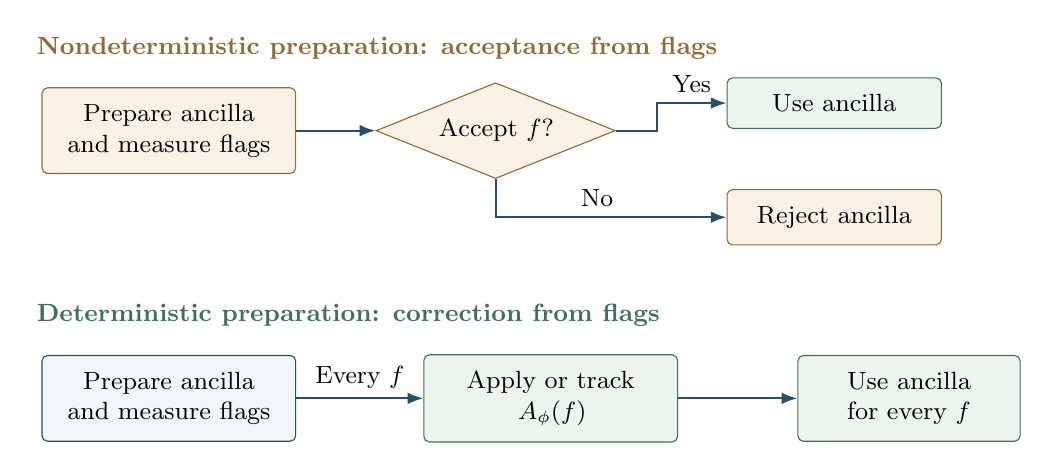
\begin{tikzpicture}[>=Latex,font=\small]
 \node[anchor=west,font=\small\bfseries,text=ochre] at (-1.8,.8)
   {Nondeterministic preparation: acceptance from flags};
 \node[prior,text width=2.8cm] (p) at (0,-.25)
   {Prepare ancilla\\and measure flags};
 \node[decision,text width=1.6cm,draw=ochre,fill=ochrewash]
   (f) at (4.15,-.25) {Accept $f$?};
 \node[good,text width=2.3cm] (yes) at (8.45,.1)
   {Use ancilla};
 \node[prior,text width=2.3cm] (no) at (8.45,-1.35)
   {Reject ancilla};
 \draw[flow] (p)--(f);
 \draw[flow] (f.east)--(6.2,-.25)|-node[pos=.75,above]{Yes}(yes.west);
 \draw[flow] (f.south)|-node[pos=.72,above]{No}(no.west);
 \node[anchor=west,font=\small\bfseries,text=green] at (-1.8,-2.6)
   {Deterministic preparation: correction from flags};
 \node[card,text width=2.8cm] (dp) at (0,-3.65)
   {Prepare ancilla\\and measure flags};
 \node[good,text width=2.8cm] (frame) at (4.85,-3.65)
   {Apply or track\\$A_\phi(f)$};
 \node[good,text width=2.4cm] (use) at (9.4,-3.65)
   {Use ancilla\\for every $f$};
 \draw[flow] (dp)--node[above,font=\small]{Every $f$}(frame);
 \draw[flow] (frame)--(use);
\end{tikzpicture}
\caption{The preparation task changes from deciding which ancillas to
accept to supplying a correction for every flag record. Equation
\eqref{eq:detprep} states the residual-error guarantee of the deterministic
construction.}
\label{fig:detprep}
\end{figure}

\begin{remark}[Frames and protection order]
The correction $A_\phi(f)$ is tracked through the transversal CNOT and
readout, producing known updates to the data frame and processed syndrome.
For a preparation with $q$ faults, \eqref{eq:detprep} gives a residual
bound of $q$, even if that preparation was designed for a larger order $b$.
The same correction works for every history sharing the flags. A related
flag-dependent residual-error condition for syndrome circuits appears in
\cite[Definition~2]{chao}.
\end{remark}

\begin{definition}[Preparation family and distance labels]
For each $b=0,\ldots,t$, let the library supply a deterministic preparation
of the appropriate ancilla state satisfying $\DPrep_\phi(b)$.
Write $\delta_{\mathrm{det}}(b)$ for the label of a least-cost such
preparation. A family with the distance assignment
\begin{equation}
 \text{label }2b+1\quad\Longrightarrow\quad\DPrep_\phi(b)
 \label{eq:distancecontract}
\end{equation}
will be called a deterministic preparation family with the stated distance
guarantee.
\end{definition}

\begin{definition}[Component syndrome decoders]
Choose $D_X,D_Z$ such that
\[
 H_ZD_X(\sigma)=\sigma,\qquad H_XD_Z(\tau)=\tau
\]
for every attainable syndrome, and such that they correct every component
error of weight at most $t$ modulo the corresponding component stabilizer.
On all other syndromes, select any representative with that syndrome.
\end{definition}

\begin{construction}[The deterministic two-extraction cycle]
\label[construction]{con:two}
\mbox{}
\begin{enumerate}
 \item Run Z-SE using a $\DPrep_{\overline{+^k}}(t)$ preparation.
 Track $A_{\overline{+^k}}(f_1)$ and store the adjusted syndrome $\sigma_Z$.
 \item Obtain a certified lower bound $L$ on spent faults from the first
 record. Run X-SE using a
 $\DPrep_{\overline{0^k}}(t-L)$ preparation, track its assigned correction,
 and store the adjusted syndrome $\sigma_X$.
 \item Complete the cycle with
 \[
 C=X(D_X(\sigma_Z))Z(D_Z(\sigma_X))
 \]
 in the tracked frame.
\end{enumerate}
\end{construction}

\Needspace{10\baselineskip}
\begin{theorem}[Two-extraction deterministic Steane QEC]
\label[theorem]{thm:two}
In the preparation-fault model, \cref{con:two} satisfies EC A and EC B.
\end{theorem}
\begin{proof}
Let the preparations contain $q_1,q_2$ faults, with $s=q_1+q_2\leq t$.
By certification, $q_1\geq L$, and hence
\[
 q_2\leq t-q_1\leq t-L.
\]
Both deterministic-preparation guarantees apply. Denote the residual
ancilla supports after their assigned corrections by $x_i,z_i$.
Then $\wt(x_i),\wt(z_i)\leq q_i$, and
\cref{lem:two-transitions} holds in the tracked frame.

Set $c_X=D_X(\sigma_Z)$ and $c_Z=D_Z(\sigma_X)$. The decoder syndrome
equations give
\[
 n_X=u+x_1+c_X\in\ker H_Z,\qquad
 n_Z=v+z_1+z_2+c_Z\in\ker H_X.
\]
The corrected data Pauli is therefore, up to phase,
\begin{equation}
 X(u+x_2+c_X)Z(v+z_1+c_Z)
 =X(x_1+x_2)Z(z_2)\,X(n_X)Z(n_Z).
 \label{eq:tworesidual}
\end{equation}
The last factor is in $\Norm$, and the first has CSS weight at most
$q_1+q_2=s$. This proves EC A for every incoming $u,v$.

If $r+s\leq t$, the effective measured errors satisfy
\[
 \wt(u+x_1)\leq r+q_1\leq t,\qquad
 \wt(v+z_1+z_2)\leq r+q_1+q_2\leq t.
\]
The component decoders then make $X(n_X)$ and $Z(n_Z)$ stabilizers.
Equation \eqref{eq:tworesidual} has $\nu\leq s$, proving EC B.
\end{proof}

\begin{corollary}[Adaptive preparation distance]
\label[corollary]{cor:drop}
For a deterministic preparation family satisfying
\eqref{eq:distancecontract}, the two-extraction cycle may use
\begin{equation}
 \boxed{\delta_1=d,\qquad
        \delta_2=2(t-L)+1=d-2L.}
 \label{eq:drop}
\end{equation}
\end{corollary}
\begin{proof}
The first preparation tolerates $t$ faults. By \cref{lem:budget}, the
second needs protection through $t-L$ faults. Apply the family's distance
assignment.
\end{proof}

\begin{figure}[H]
\centering
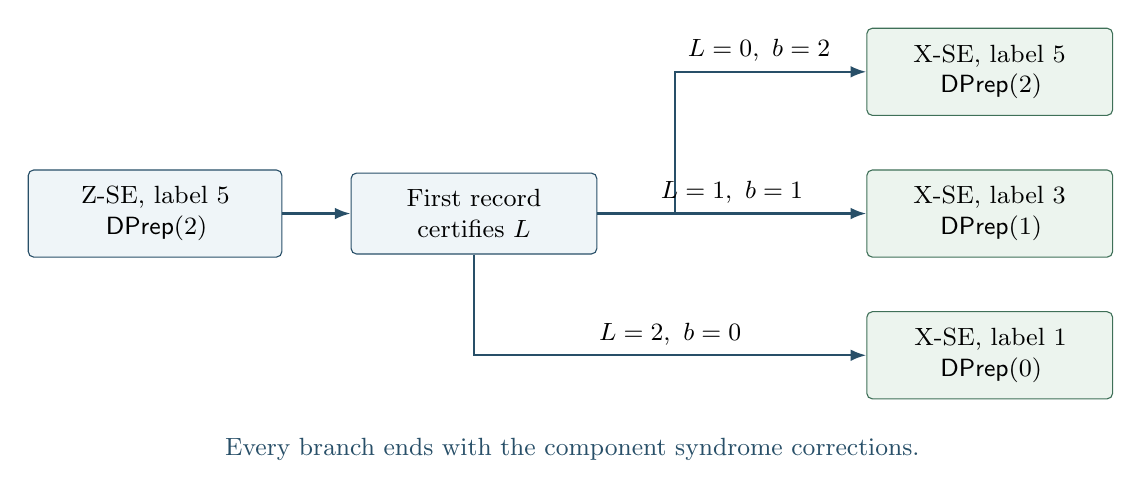
\begin{tikzpicture}[>=Latex,font=\small]
 \node[card,text width=2.8cm,minimum height=1cm] (z) at (0,0)
   {Z-SE, label $5$\\$\DPrep(2)$};
 \node[card,text width=2.7cm,minimum height=1cm] (r) at (4.05,0)
   {First record\\certifies $L$};
 \node[good,text width=2.7cm] (x5) at (10.6,1.8)
   {X-SE, label $5$\\$\DPrep(2)$};
 \node[good,text width=2.7cm] (x3) at (10.6,0)
   {X-SE, label $3$\\$\DPrep(1)$};
 \node[good,text width=2.7cm] (x1) at (10.6,-1.8)
   {X-SE, label $1$\\$\DPrep(0)$};
 \draw[flow] (z)--(r);
 \draw[flow] (r.east)--(6.6,0)|-node[pos=.72,above]{$L=0,\ b=2$}(x5.west);
 \draw[flow] (r.east)--node[above]{$L=1,\ b=1$}(x3.west);
 \draw[flow] (r.south)|-node[pos=.75,above]{$L=2,\ b=0$}(x1.west);
 \node[font=\small,text=accent,align=center] at (5.3,-3.0)
   {Every branch ends with the component syndrome corrections.};
\end{tikzpicture}
\caption{A distance-five example of \cref{cor:drop}. The first record
selects the protection needed by the second deterministic preparation.
The data code and syndrome decoders retain distance five throughout.}
\label{fig:distance}
\end{figure}

\begin{remark}[Why the distance decreases]
The first preparation's residual errors remain in
\eqref{eq:tworesidual}. Their weights have already been bounded by $q_1$,
and the code's original radius handles them together with the incoming
error and the second stage's faults. The bound $L$ reduces only the order
of new faults that the second preparation must tolerate.
When $L=t$, that preparation is required to work without new faults.
\end{remark}
\FloatBarrier

\section{Complete noisy extractions}
\label{sec:fullnoise}

\begin{definition}[Stage response]
After tracking its preparation correction, represent the first complete
stage by
\begin{equation}
 \sigma_Z=H_Z(u+\beta_1),\qquad
 E_D^{(1)}=X(u+\alpha_1)Z(v+\gamma_1),
 \label{eq:genZ}
\end{equation}
and the second by
\begin{equation}
 \begin{split}
 \sigma_X&=H_X(v+\gamma_1+\beta_2),\\
 E_D^{(2)}&=X(u+\alpha_1+\gamma_2)Z(v+\gamma_1+\alpha_2).
 \end{split}
 \label{eq:genX}
\end{equation}
A stage has the required response bound through order $b$ if every
$q_i\leq b$ faulty locations give
\begin{equation}
 \wt(\beta_i)\leq q_i,\qquad
 \wt(\alpha_i+\beta_i)\leq q_i,\qquad
 \wt(\gamma_i)\leq q_i.
 \label{eq:localeffect}
\end{equation}
The count includes preparation, coupling, readout, and scheduled data idles.
\end{definition}

\begin{remark}[Meaning of the response variables]
The vector $\beta_i$ describes the measured error shift,
$\alpha_i+\beta_i$ the residual in that component after syndrome
correction, and $\gamma_i$ the component introduced into the data and
diagnosed by the other basis. In the preparation-fault model,
\[
 (\alpha_1,\beta_1,\gamma_1)=(0,x_1,z_1),\qquad
 (\alpha_2,\beta_2,\gamma_2)=(0,z_2,x_2).
\]
For a transversal faulty location, its readout and data effects are on the
same data coordinate, motivating the joint bound on
$\alpha_i+\beta_i$.
\end{remark}

\begin{corollary}[Two complete stages]
\label[corollary]{cor:fullnoise}
If the two stages satisfy \eqref{eq:genZ}--\eqref{eq:localeffect}
through orders $t$ and $t-L$, respectively, the deterministic
two-extraction cycle satisfies EC A and EC B with faults at every
modeled location. Here $L$ bounds faults in the completed first stage.
\end{corollary}
\begin{proof}
After the component syndrome corrections, the residual differs by a
normalizer from
\[
 X(\alpha_1+\beta_1+\gamma_2)Z(\alpha_2+\beta_2),
\]
whose CSS weight is at most $q_1+q_2$. This proves EC A.
Under $r+q_1+q_2\leq t$, the measured errors $u+\beta_1$ and
$v+\gamma_1+\beta_2$ have weights at most $r+q_1$ and
$r+q_1+q_2$. The decoders make the normalizer a stabilizer, proving EC B.
\end{proof}

\section{Selecting the minimal next action}
\label{sec:minimal}

The deterministic construction gives a short protocol directly. We now
return to the general history set and choose the least costly continuation
available from a specified circuit library.

\begin{definition}[Continuation and outcome]
For a compatible set $H$ and action $a$, let $T(H,a,o)$ contain every
extension of its histories that produces the new outcome $o$ and has
$q_h+|G|\leq t$, where $G$ is the new fault history.
Its data Pauli and fault count are updated, and its EC B condition is
$r_h+q_h+|G|\leq t$. This is \cref{con:update} applied to the full
selected extraction.
\end{definition}

\begin{definition}[The optimization problem]
Fix a finite library $\mathscr A$ of extraction actions, a positive
resource cost $c(a)$ for each action, and a cap of $K$ further
extractions. We minimize the worst-case total remaining cost of a
nonpostselected continuation with terminal Pauli-frame corrections.
Examples of $c(a)$ are CNOT count, noisy location count, and duration.
The first action $(Z,d)$ is fixed.
\end{definition}

\begin{construction}[Backward recursion for the policy]
\label[construction]{con:bellman}
For nonempty compatible sets $H$, let $\Safe(H)$ denote the safe
intersection in \eqref{eq:safe}. Define
\begin{align}
 V_0(H)&=
 \begin{cases}
 0,&\Safe(H)\ne\varnothing,\\
 +\infty,&\Safe(H)=\varnothing,
 \end{cases}\label{eq:base}\\
 V_j(H)&=
 \begin{cases}
 0,&\Safe(H)\ne\varnothing,\\[2pt]
 \displaystyle\min_{a\in\mathscr A}
 \left[c(a)+\max_{o:T(H,a,o)\ne\varnothing}
                 V_{j-1}(T(H,a,o))\right],&\text{otherwise}.
 \end{cases}\label{eq:bellman}
\end{align}
At a nonterminal state with finite value, store an action attaining the
minimum. At a terminal state, store a correction from $\Safe(H)$.
\end{construction}

\begin{remark}[The scope of minimality]
The value $V_j$ minimizes total remaining work for the specified library
and extraction cap. Consequently, it includes the cost of any additional
measurements needed after a cheaper first continuation.
All possible bounded-fault outcomes appear in the maximum.
\end{remark}

\begin{figure}[H]
\centering
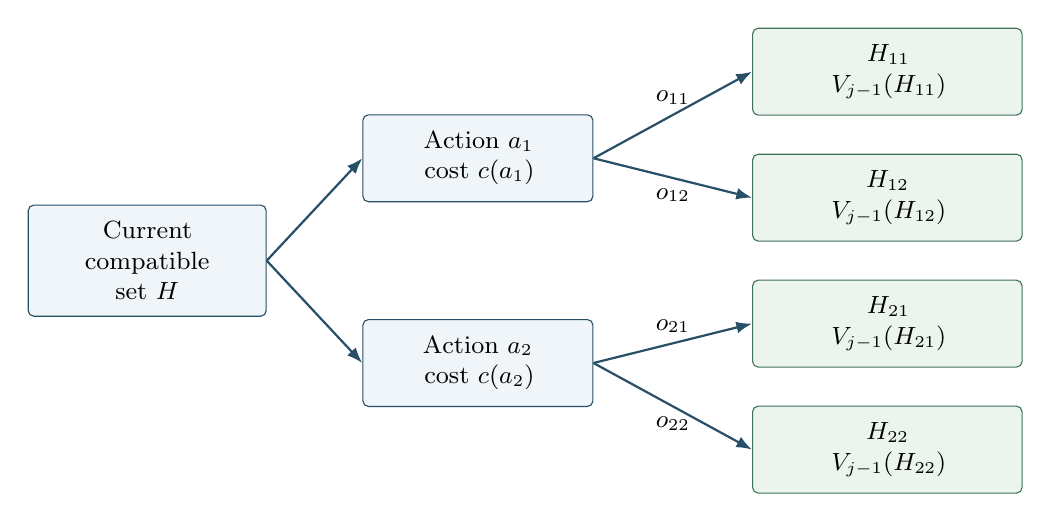
\begin{tikzpicture}[>=Latex,font=\small]
 \node[card,text width=2.6cm] (root) at (0,0)
   {Current compatible\\set $H$};
 \node[card,text width=2.5cm] (a) at (4.2,1.3)
   {Action $a_1$\\cost $c(a_1)$};
 \node[card,text width=2.5cm] (b) at (4.2,-1.3)
   {Action $a_2$\\cost $c(a_2)$};
 \node[good,text width=3.0cm] (a1) at (9.4,2.4)
   {$H_{11}$\\$V_{j-1}(H_{11})$};
 \node[good,text width=3.0cm] (a2) at (9.4,.8)
   {$H_{12}$\\$V_{j-1}(H_{12})$};
 \node[good,text width=3.0cm] (b1) at (9.4,-.8)
   {$H_{21}$\\$V_{j-1}(H_{21})$};
 \node[good,text width=3.0cm] (b2) at (9.4,-2.4)
   {$H_{22}$\\$V_{j-1}(H_{22})$};
 \draw[flow] (root.east)--(a.west);
 \draw[flow] (root.east)--(b.west);
 \draw[flow] (a.east)--node[above]{$o_{11}$}(a1.west);
 \draw[flow] (a.east)--node[below]{$o_{12}$}(a2.west);
 \draw[flow] (b.east)--node[above]{$o_{21}$}(b1.west);
 \draw[flow] (b.east)--node[below]{$o_{22}$}(b2.west);
\end{tikzpicture}
\caption{Comparing two candidate actions, each illustrated with two
compatible outcomes. For each action, add its cost to the largest child
value; then choose the smaller total. The child sets already include
faults during that action. This is the recursion in
\cref{con:bellman}.}
\label{fig:minimal}
\end{figure}

\begin{construction}[Online adaptive cycle]
\label[construction]{con:online}
Run $(Z,d)$ and then repeat the following:
\begin{enumerate}
 \item Record the flags and syndrome and update $\Hist(R)$.
 \item If $\Safe(R)\ne\varnothing$, use its stored correction and finish.
 \item Otherwise run the continuation stored by \cref{con:bellman}.
\end{enumerate}
This is the controller in \cref{fig:controller}.
\end{construction}

\begin{theorem}[Correctness, termination, and minimality]
\label[theorem]{thm:general}
Suppose every nonempty child of the initial $(Z,d)$ action has finite
value $V_K$. Then \cref{con:online} terminates within $K+1$
extractions and satisfies EC A and EC B.
Among policies with the same library, initial action, extraction cap,
terminal corrections, and cost objective, it has minimum worst-case cost.
\end{theorem}
\begin{proof}
For any execution with at most $t$ faults, \cref{lem:true} retains the
true history. A finite value in \eqref{eq:bellman} selects an action for
which every nonempty child has finite value. The remaining extraction
count decreases by one at each step. Thus the cycle reaches a terminal
state within the cap. Its stored correction belongs to $\Safe(R)$ and
satisfies both EC conditions by \cref{prop:stop}.

For minimality, a nonterminal policy chooses a first action and must
handle each of its compatible outcomes. Inductively, its worst remaining
child cost is at least the maximum in \eqref{eq:bellman}. Minimization
over the first action attains this bound.
\end{proof}

\begin{remark}[Completing the decision table]
The table is finite. For records with an empty bounded-history set, assign
a fixed correction and finish at or before the same extraction cap.
\end{remark}

\section{Fault-charging bounds and expected extraction counts}
\label{sec:counts}

\begin{definition}[Gadgets and rounds]
One SE gadget is one extraction in a single basis. A paired round consists
of a Z-SE followed by an X-SE, using the preparations chosen by the
protocol. Write $N$ for the number of individual gadgets and $J$ for the
number of rounds. A schedule executing both gadgets in each round has
$N=2J$.
\end{definition}

\begin{definition}[Fault-charged round policy]
\label[definition]{def:charged}
A certified round policy finishes only with a correction from $\Safe(R)$.
Every round after which it continues satisfies
\begin{equation}
 L(R_{\mathrm{after}})\geq L(R_{\mathrm{before}})+1.
 \label{eq:roundprogress}
\end{equation}
A sufficient certificate for \eqref{eq:roundprogress} is a nonzero
preparation flag in that fresh round, independent of the data and with
fault-free value zero. Every compatible history then contains at least
one new internal fault. This policy uses all measured ancillas and retains
the observations from earlier rounds.
\end{definition}

\begin{proposition}[Worst-case round count]
\label[proposition]{prop:roundbound}
For a fault-charged round policy with $s\leq t$ total faults,
\begin{equation}
 \boxed{J\leq s+1\leq t+1
              =1+\left\lfloor\frac d2\right\rfloor.}
 \label{eq:roundbound}
\end{equation}
If a round uses at most two gadgets, then
\begin{equation}
 \boxed{N\leq 2(s+1)\leq 2(t+1)=d+1.}
 \label{eq:gadgetbound}
\end{equation}
\end{proposition}
\begin{proof}
The first $J-1$ rounds all continue. By
\eqref{eq:roundprogress}, their observations certify at least $J-1$
faults. The true history has at most $s$ faults, so $J-1\leq s$.
Each round contributes at most two gadgets.
The same argument rules out an unfinished $(s+1)$st round, establishing
termination within the bound.
\end{proof}

\begin{remark}[The progress condition]
The role of code distance is to supply the total budget $t$.
The round policy supplies the progress statement
\eqref{eq:roundprogress}. Together they prove the proposed
$1+\lfloor d/2\rfloor$ bound on paired rounds.
A quiet first Z-SE can still require X-SE, since both syndrome components
are needed. Counting individual gadgets therefore retains the initial
two-gadget cycle.
\end{remark}

\begin{definition}[No-flag and direct-use acceptance rates]
\label[definition]{def:AR}
For a chosen stochastic fault model and a gadget in basis $B$ with circuit
label $\delta$, define
\begin{equation}
 \operatorname{AR}^{0}_{B,\delta}
    =\Pr(f_{B,\delta}=0).
 \label{eq:ARzero}
\end{equation}
Let $G_{B,\delta}$ be the event that the preparation record passes its
prescribed direct-use test, supplying the required ancilla-error bound
within its protection order without another diagnostic extraction.
Its direct-use acceptance rate is
\begin{equation}
 a_{B,\delta}=\Pr(G_{B,\delta}).
 \label{eq:ARdirect}
\end{equation}
For the earlier nondeterministic preparation rule, take
$G_{B,\delta}=\{f_{B,\delta}=0\}$, giving
$a_{B,\delta}=\operatorname{AR}^{0}_{B,\delta}$.
For deterministic state preparation, every flag record has its assigned
correction, so $a_{B,\delta}=1$.
\end{definition}

\begin{remark}[The deterministic value one]
The equality $a_{B,\delta}=1$ expresses completion of the deterministic
preparation for every flag outcome. The raw flag probability
$\operatorname{AR}^{0}_{B,\delta}$ describes a different event.
In the resource formulas below, the acceptance rate is the direct-use
rate $a_{B,\delta}$. The two rates coincide for the earlier no-flag
acceptance test.
\end{remark}

\begin{proposition}[Theoretical calculation of each no-flag rate]
Let the gadget's elementary locations be indexed by $\ell$, with local
fault variable $e_\ell$ and distribution $p_\ell(e_\ell)$, including the
no-fault value. If these variables are independent, then
\begin{equation}
 \operatorname{AR}^{0}_{B,\delta}
 =\sum_{\mathbf e:\,f_{B,\delta}(\mathbf e)=0}
             \ \prod_\ell p_\ell(e_\ell).
 \label{eq:ARsum}
\end{equation}
The direct-use rate is obtained by replacing the summation condition by
$\mathbf e\in G_{B,\delta}$.
\end{proposition}
\begin{proof}
Each complete local-fault assignment has probability
$\prod_\ell p_\ell(e_\ell)$. Summing the assignments producing the
specified event gives its probability.
\end{proof}

\begin{definition}[Expected count for a fixed adaptive policy]
Fix the stochastic model and a finite policy $\pi$.
Let $p(o\mid R,a)$ be the conditional probability of the next complete
outcome, including flags and syndrome, and let $\mathcal E_\pi(R)$ be the
expected number of additional SE gadgets. Then
\begin{equation}
 \mathcal E_\pi(R)=
 \begin{cases}
 0,&R\text{ is a terminal record},\\[2pt]
 \displaystyle 1+\sum_o p(o\mid R,a_\pi(R))
                    \mathcal E_\pi(Ro),&\text{otherwise}.
 \end{cases}
 \label{eq:expectedpolicy}
\end{equation}
Here $Ro$ is the record extended by the chosen gadget and its outcome.
\end{definition}

\begin{proposition}[Expected-cost recursion]
Equation \eqref{eq:expectedpolicy} gives the exact expected gadget
count of the policy. Replacing the leading $1$ by $c(a_\pi(R))$
gives its expected resource cost.
\end{proposition}
\begin{proof}
A nonterminal action executes one gadget. Conditioning its remaining
cost on each next outcome gives the sum. The recursion terminates at
the finite policy's leaves.
\end{proof}

\begin{remark}[When acceptance rates suffice]
If all non-direct outcomes use the same continuation, their probabilities
combine into the single factor $1-a_{B,\delta}$. When different flag
patterns select different distances or bases, their probabilities enter
\eqref{eq:expectedpolicy} separately. Both cases use the same
conditional-expectation calculation.
\end{remark}

\begin{construction}[A unit-decrement round ladder]
\label[construction]{con:ladder}
Consider a certified paired-round policy whose continuation depends on a
remaining budget index $b$. The round at index $b$ uses preparations with
label $\delta_b$. It finishes when both preparations meet their direct-use
conditions. Otherwise it continues at $b-1$, retaining all previous
records. The round at $b=0$ completes the capped schedule.
Each continuing round certifies at least one new fault, as in
\cref{def:charged}.

Let
\begin{equation}
 A_b=\Pr(\text{both direct-use conditions}\mid
                   \text{round }b\text{ reached}),\qquad
 Q_b=1-A_b.
 \label{eq:roundacceptance}
\end{equation}
When preparation outcomes are independent and their direct-use rates
depend only on basis and label,
\begin{equation}
 A_b=a_{Z,\delta_b}\,a_{X,\delta_b}.
 \label{eq:roundARproduct}
\end{equation}
If the two bases have the same rate $a_{\delta_b}$, this reduces to
$A_b=a_{\delta_b}^{\,2}$. A family with certified choices
$\delta_b=2b+1$ gives the distance ladder $d,d-2,\ldots,1$.
\end{construction}

\begin{proposition}[Expected number on the round ladder]
\label[proposition]{prop:ladderexpectation}
Let $M_b$ be the expected number of gadgets still to execute at the start
of round $b$ in \cref{con:ladder}, conditional on reaching that round. Then
\begin{equation}
 M_0=2,\qquad M_b=2+Q_bM_{b-1}\quad(b\geq1),
 \label{eq:roundexpectedrec}
\end{equation}
and hence
\begin{equation}
 \boxed{M_t=2\left(1+Q_t+Q_tQ_{t-1}
                      +\cdots+\prod_{b=1}^{t}Q_b\right).}
 \label{eq:roundexpected}
\end{equation}
In particular, $2\leq M_t\leq2(t+1)$.
\end{proposition}
\begin{proof}
Each reached round uses two gadgets and reaches the next round with
probability $Q_b$. This proves \eqref{eq:roundexpectedrec}.
Repeated substitution gives \eqref{eq:roundexpected}; each product lies
between zero and one.
\end{proof}

\begin{remark}[Earlier safe stopping]
The general controller can also finish at flagged records whose common
correction set is nonempty. Using those additional terminal records can
reduce the ladder's expected count. Equation
\eqref{eq:expectedpolicy} evaluates the resulting policy.
\end{remark}

\begin{figure}[H]
\centering
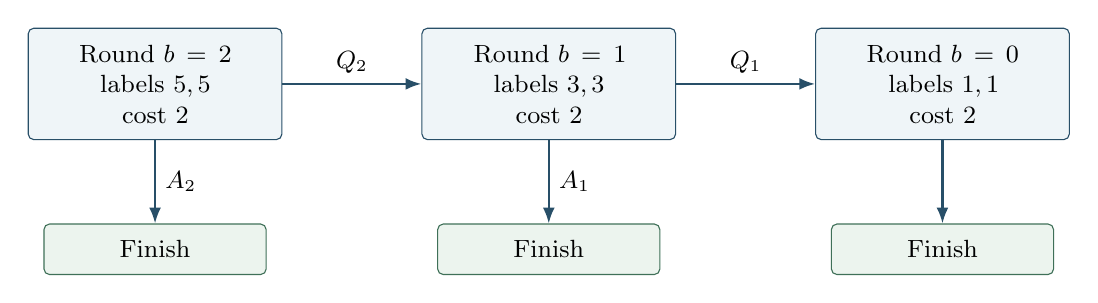
\begin{tikzpicture}[>=Latex,font=\small]
 \node[card,text width=2.8cm,minimum height=1.1cm] (r2) at (0,0)
   {Round $b=2$\\labels $5,5$\\cost $2$};
 \node[card,text width=2.8cm,minimum height=1.1cm] (r1) at (5,0)
   {Round $b=1$\\labels $3,3$\\cost $2$};
 \node[card,text width=2.8cm,minimum height=1.1cm] (r0) at (10,0)
   {Round $b=0$\\labels $1,1$\\cost $2$};
 \node[good,text width=2.4cm] (s2) at (0,-2.1) {Finish};
 \node[good,text width=2.4cm] (s1) at (5,-2.1) {Finish};
 \node[good,text width=2.4cm] (s0) at (10,-2.1) {Finish};
 \draw[flow] (r2)--node[above]{$Q_2$}(r1);
 \draw[flow] (r1)--node[above]{$Q_1$}(r0);
 \draw[flow] (r2)--node[right]{$A_2$}(s2);
 \draw[flow] (r1)--node[right]{$A_1$}(s1);
 \draw[flow] (r0)--(s0);
\end{tikzpicture}
\caption{A distance-five round ladder under the stated continuation
certification. The three rounds are reached with probabilities
$1,Q_2,Q_2Q_1$, respectively, giving
$M_2=2(1+Q_2+Q_2Q_1)$. Every prepared ancilla is used.}
\label{fig:roundladder}
\end{figure}

\begin{corollary}[Equal-rate and deterministic limits]
If every round has the same completion probability $A>0$, then
\begin{equation}
 M_t=2\sum_{j=0}^{t}(1-A)^j
    =\frac{2\bigl[1-(1-A)^{t+1}\bigr]}{A}.
 \label{eq:constAR}
\end{equation}
For deterministic preparations, $a_{Z,\delta}=a_{X,\delta}=1$, so
$A=1$ and $M_t=2$. This agrees with the deterministic two-extraction
construction in \cref{thm:two}.
\end{corollary}
\begin{proof}
The equal-rate case is a finite geometric sum.
With deterministic preparations the first round meets both direct-use
conditions and the cycle finishes after its two gadgets.
\end{proof}

\begin{remark}[A single-gadget repair chain]
A policy can use a finer unit than a paired round. For a certified chain
that runs one gadget per step, continues at $b-1$ on a non-direct outcome,
and finishes at $b=0$, its expected length obeys
\[
 g_0=1,\qquad g_b=1+(1-a_b)g_{b-1}.
\]
The chain has at most $t+1$ gadgets. If a complete certified QEC policy
consists of this chain and one fixed dual-basis extraction, its total is
$N\leq t+2$ and $\mathbb E[N]=1+g_t$. Thus the gadget bound follows the
chosen repair policy, while the two-gadget deterministic limit is the
same.
\end{remark}
\FloatBarrier

\section{Applying the construction to the preparation circuits}
\label{sec:application}

\begin{definition}[Syndrome-assisted preparation correction]
A preparation has a syndrome-assisted correction through order $b$ if
the pair of its flags and a perfect syndrome of its boundary error
determines a correction for every history of at most $b$ faults.
This is the operational correction property assumed for the earlier
distance-$d$ preparations.
\end{definition}

\begin{remark}[Where the preparation information is used]
A deterministic preparation supplies its correction from the available
preparation record $f$, as in \cref{def:detprep}.
A syndrome-assisted preparation also uses a later syndrome to choose its
correction. In a Steane cycle, that later observation is
$H_X(v+z_1+z_2)$ or $H_Z(u+x_1)$.
The compatible-history update keeps the incoming-error, preparation-error,
and shared fault-budget constraints together while interpreting those
observations.
\end{remark}

\begin{construction}[A protocol for the supplied family]
For each available preparation, tabulate the possible responses
$(\ell,f,\xi,\zeta)$, or the corresponding complete noisy stage responses.
Then:
\begin{enumerate}
 \item Use \cref{con:update} to form the compatible sets after the initial
 Z-SE and its candidate continuations.
 \item Compute the common correction set \eqref{eq:safe} at each record.
 \item Fix a cost and extraction cap, evaluate \cref{con:bellman}, and
 install each minimizing action and terminal correction in the controller.
 \item Assign probabilities to the responses under a chosen stochastic
 fault model and evaluate \eqref{eq:expectedpolicy} for the expected
 gadget count.
\end{enumerate}
Whenever the initial children have finite values, \cref{thm:general}
gives a nonpostselected protocol with the stated minimality.
For a deterministic preparation family,
\cref{con:two,cor:drop} already supply a two-extraction policy; the
same optimization can refine its individual branches.
\end{construction}

\begin{remark}[The resulting mathematical task]
For the earlier nondeterministic preparations, the remaining task is to
construct the response tables and the finite continuation policy.
For a deterministic family, it is to supply the maps $A_\phi(f)$ and
their guarantees \eqref{eq:detprep}. In both cases the cycle finishes
as soon as its complete record admits one common safe correction.
\end{remark}

\begin{thebibliography}{9}
\bibitem{gottesman}
D.~Gottesman,
\emph{An Introduction to Quantum Error Correction and Fault-Tolerant
Quantum Computation}, arXiv:0904.2557 (2009).
\href{https://arxiv.org/abs/0904.2557}{arxiv.org/abs/0904.2557}.
Definition~5 gives the EC conditions; Sec.~4.4 discusses Steane extraction.

\bibitem{chao}
R.~Chao and B.~W.~Reichardt,
\emph{Flag fault-tolerant error correction for any stabilizer code},
arXiv:1912.09549 (2019).
\href{https://arxiv.org/abs/1912.09549}{arxiv.org/abs/1912.09549}.
Definitions~1--2 give full EC conditions and a flag-dependent
residual-error condition for syndrome circuits.
\end{thebibliography}
\end{document}
